% node_circulator_ring.tex — Fork-A 3-port circulator ring (Vol 9 Ch.3 / 03a)
% Included from chapters/03a_device_circuit_models.tex
% Renders the Fork-A resolution of src/scripts/vol_9_device/node_circulator_coupling.py:
% LEFT = the 2-port skew (reciprocal = optical-activity GYRATOR, not one-way);
% RIGHT = the 3-port RING (EM/photon as the 3rd leg) needed for genuine
% chiral non-reciprocity; loop phase 3χθ_χ flips with χ but magnitude IMPOSED.
% Pure TikZ; not a driver plot.
\begin{figure}[htbp]
\centering
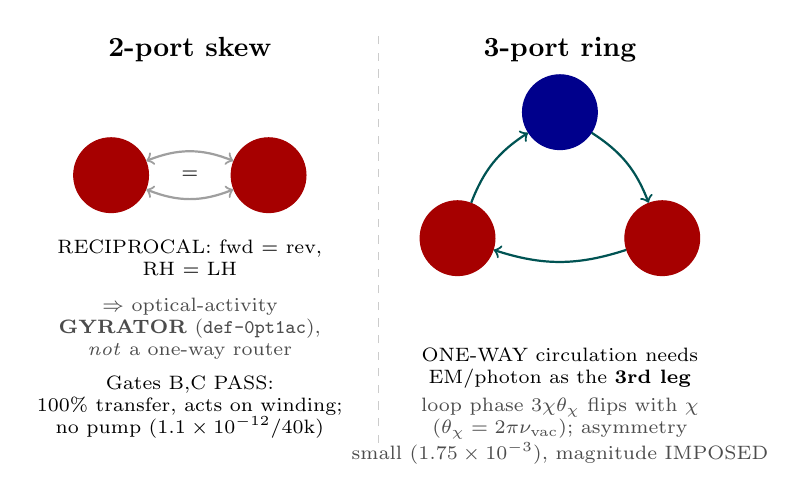
\begin{tikzpicture}[scale=1.0, transform shape, font=\footnotesize,
    port/.style={circle, draw, fill=black!7, minimum size=0.95cm, inner sep=0pt}]

    % ===== LEFT: the 2-port reciprocal skew (gyrator) =====
    \begin{scope}[shift={(0,0)}]
        \node[font=\bfseries] at (1.0,2.6) {2-port skew};
        \node[port, red!65!black] (s2) at (0,1.0) {shear};
        \node[port, red!65!black] (b2) at (2.0,1.0) {bulk};
        \draw[<->, thick, gray!75] (s2) to[bend left=22] (b2);
        \draw[<->, thick, gray!75] (b2) to[bend left=22] (s2);
        \node[align=center, font=\scriptsize] at (1.0,1.0) {$=$};
        \node[align=center, font=\scriptsize] at (1.0,-0.05)
            {RECIPROCAL: fwd $=$ rev,\\ RH $=$ LH};
        \node[align=center, font=\scriptsize, gray!60!black] at (1.0,-0.95)
            {$\Rightarrow$ optical-activity\\ \textbf{GYRATOR} (\texttt{def-0pt1ac}),\\ \emph{not} a one-way router};
        \node[align=center, font=\scriptsize] at (1.0,-1.95)
            {Gates B,C PASS:\\ 100\% transfer, acts on winding;\\ no pump ($1.1\times10^{-12}$/40k)};
    \end{scope}

    % divider
    \draw[gray!40, dashed] (3.4,-2.4) -- (3.4,2.8);

    % ===== RIGHT: the 3-port ring (EM as 3rd leg) =====
    \begin{scope}[shift={(5.7,0.6)}]
        \node[font=\bfseries] at (0,2.0) {3-port ring};
        \node[port, red!65!black] (s3) at (-1.3,-0.4) {shear};
        \node[port, red!65!black] (b3) at (1.3,-0.4) {bulk};
        \node[port, blue!55!black] (e3) at (0,1.2) {EM};
        % one-way circulation arrows
        \draw[->, thick, teal!65!black] (s3) to[bend left=18] (e3);
        \draw[->, thick, teal!65!black] (e3) to[bend left=18] (b3);
        \draw[->, thick, teal!65!black] (b3) to[bend left=18] (s3);
        \node[teal!55!black, font=\scriptsize] at (0,0.15) {$\circlearrowleft$};
    \end{scope}
    \node[align=center, font=\scriptsize] at (5.7,-1.45)
        {ONE-WAY circulation needs\\ EM/photon as the \textbf{3rd leg}};
    \node[align=center, font=\scriptsize, gray!60!black] at (5.7,-2.25)
        {loop phase $3\chi\theta_\chi$ flips with $\chi$\\ ($\theta_\chi=2\pi\nu_{\mathrm{vac}}$); asymmetry\\ small ($1.75\times10^{-3}$), magnitude IMPOSED};

\end{tikzpicture}
\caption{Fork-A coupling resolution (rendering \kbleaf{src/scripts/vol\_9\_device/node\_circulator\_coupling.py}, verdict PARTIAL). A conservative skew-Hermitian shear$\leftrightarrow$bulk coupling \emph{exists} and escapes the graft-v3 trilinear dead-end (no pump, not isolation, not inert --- Gates B/C pass, 100\% helicity transfer). \emph{Left:} but the 2-port skew is \textbf{RECIPROCAL} (forward $=$ reverse, RH $=$ LH) --- it \emph{is} the reciprocal optical-activity \textbf{gyrator} (\texttt{def-0pt1ac}), not a one-way router. \emph{Right:} genuine chiral \emph{non-reciprocity} (a one-way circulator) requires the \textbf{3-port ring} with the EM/photon port as the third leg; the gauge-invariant loop phase $3\chi\theta_\chi$ ($\theta_\chi=2\pi\nu_{\mathrm{vac}}$, $\nu_{\mathrm{vac}}=2/7$) flips sign with the lattice chirality $\chi$, but the asymmetry is small ($1.75\times10^{-3}$) and the non-reciprocity \emph{magnitude} is \textbf{IMPOSED} ($\theta_\chi,\tilde\kappa$ plugged) because the cubic-FDTD engine averages chirality out --- an ECHO at the magnitude (the same FORM-deriving / VALUE-importing verdict as the rest of the node). Directional-motion$\to$mass is NEGATIVE. The coupling is $\alpha$-free throughout ($\tilde\kappa=6/5$, $\theta_\chi=2\pi\nu_{\mathrm{vac}}$). KB \kbleaf{ave-kb/vol9/ch3-pin-port-configuration/device-circuit-models.md} \S6.5.}
\label{fig:vol9_node_circulator_ring}
\end{figure}
